\documentclass[main.tex]{subfiles}
\begin{document}
\chapter{Graph Theory}

\epigraph{The origins of graph theory are humble, even frivolous.}{Norman L.\ Biggs}

\minitoc

\section{Introduction}

Graph theory is traditionally introduced using the Seven Bridges of K\"onigsberg (see fig.\ \ref{seven-bridges}). The scene is K\"onigsberg, Prussia, 1700s. Leonhard Euler\index{Leonhard Euler} sees this area -- two land masses separated by a river, with two islands in-between, all connected by 7 bridges -- and thinks, \textit{hmm, I wonder if I could walk through this city crossing each bridge only once}. Euler mathematically proved that no such walk exists due to the nature of this area. This was the birth of graph theory.

%\begin{center}
%	\begin{tikzpicture}
%% water
%\filldraw[fill=cyan,line width=0pt] (0,0) -- (0,8) -- (11.5,8) -- (11.5,0) -- cycle;
%% islands
%\filldraw[fill=gray,line width=1pt] (0,3) -- (2.5,8) -- (11.5,8) -- (10.5,6) -- (2.5,6) -- (1,3) -- cycle;
%\filldraw[fill=gray,line width=1pt] (2,3) -- (3,5) -- (7,5) -- (6,3) -- cycle;
%\filldraw[fill=gray,line width=1pt] (6.5,2) -- (8,5) -- (10.5,5) -- (9,2) -- cycle;
%\filldraw[fill=gray,line width=1pt] (0,0) -- (1,2) -- (5.5,2) -- (5,1) -- (9,1) -- (8.5,0) -- cycle;
%% bridges
%\filldraw[fill=green,line width=1pt] (3.25,4.75) -- (4,6.25) -- (4.25,6.25) -- (3.5,4.75) -- cycle;
%\filldraw[fill=green,line width=1pt] (5.25,4.75) -- (6,6.25) -- (6.25,6.25) -- (5.5,4.75) -- cycle;
%\filldraw[fill=green,line width=1pt] (8.75,4.75) -- (9.5,6.25) -- (9.75,6.25) -- (9,4.75) -- cycle;
%\filldraw[fill=green,line width=1pt] (6,3.75) -- (6.125,4) -- (8,4) -- (7.875,3.75) -- cycle;
%\filldraw[fill=green,line width=1pt] (1.75,1.75) -- (2.5,3.25) -- (2.75,3.25) -- (2,1.75) -- cycle;
%\filldraw[fill=green,line width=1pt] (3.75,1.75) -- (4.5,3.25) -- (4.75,3.25) -- (4,1.75) -- cycle;
%\filldraw[fill=green,line width=1pt] (6.75,0.75) -- (7.5,2.25) -- (7.75,2.25) -- (7,0.75) -- cycle;
%	\end{tikzpicture}
%\end{center}
\begin{figure}
	\centering
	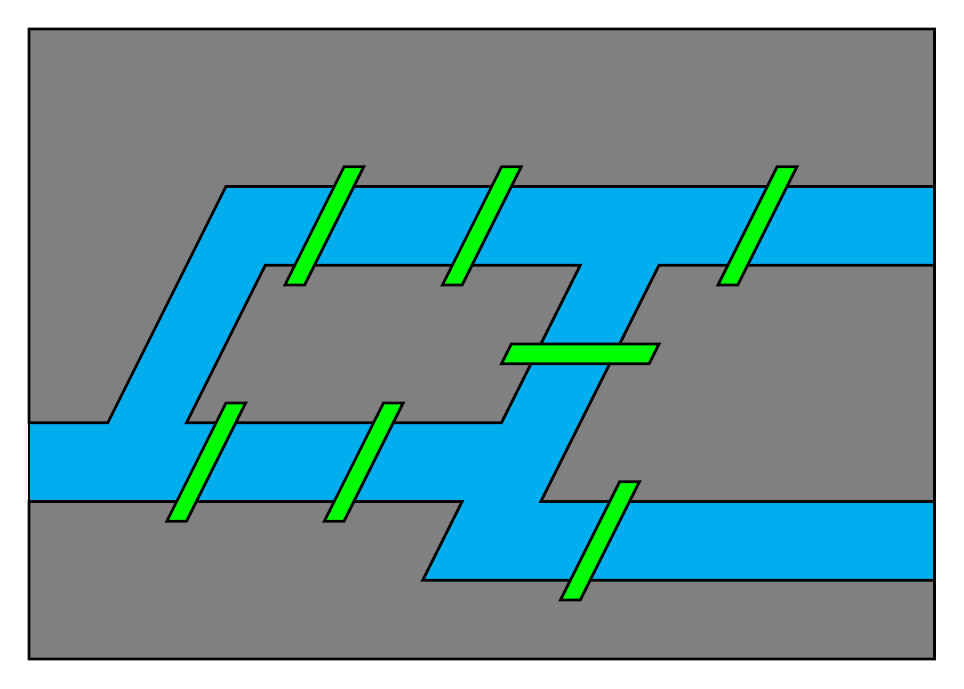
\begin{tikzpicture}
% water
\filldraw[fill=cyan,line width=1pt] (0,0) -- (0,8) -- (11.5,8) -- (11.5,0) -- cycle;
% islands
\filldraw[fill=gray,line width=1pt] (0,3) -- (0,8) -- (11.5,8) -- (11.5,6) -- (2.5,6) -- (1,3) -- cycle;
\filldraw[fill=gray,line width=1pt] (2,3) -- (3,5) -- (7,5) -- (6,3) -- cycle;
\filldraw[fill=gray,line width=1pt] (6.5,2) -- (8,5) -- (11.5,5) -- (11.5,2) -- cycle;
\filldraw[fill=gray,line width=1pt] (0,0) -- (0,2) -- (5.5,2) -- (5,1) -- (11.5,1) -- (11.5,0) -- cycle;
% bridges
\filldraw[fill=green,line width=1pt] (3.25,4.75) -- (4,6.25) -- (4.25,6.25) -- (3.5,4.75) -- cycle;
\filldraw[fill=green,line width=1pt] (5.25,4.75) -- (6,6.25) -- (6.25,6.25) -- (5.5,4.75) -- cycle;
\filldraw[fill=green,line width=1pt] (8.75,4.75) -- (9.5,6.25) -- (9.75,6.25) -- (9,4.75) -- cycle;
\filldraw[fill=green,line width=1pt] (6,3.75) -- (6.125,4) -- (8,4) -- (7.875,3.75) -- cycle;
\filldraw[fill=green,line width=1pt] (1.75,1.75) -- (2.5,3.25) -- (2.75,3.25) -- (2,1.75) -- cycle;
\filldraw[fill=green,line width=1pt] (3.75,1.75) -- (4.5,3.25) -- (4.75,3.25) -- (4,1.75) -- cycle;
\filldraw[fill=green,line width=1pt] (6.75,0.75) -- (7.5,2.25) -- (7.75,2.25) -- (7,0.75) -- cycle;
	\end{tikzpicture}
	\caption{The Seven Bridges of K\"onigsberg} \label{seven-bridges}
\end{figure}

Euler did not brute-force the solution by examining all possible paths. Instead, Euler noticed that he could abstract out the large landmasses into single points, called vertices, and connect them by simple lines, called edges, which represent the bridges. This mathematical structure is a \textit{graph}. The graph version of the Seven Bridges is presented in figure \ref{seven-bridges-graph}.

\begin{figure}
	\centering
	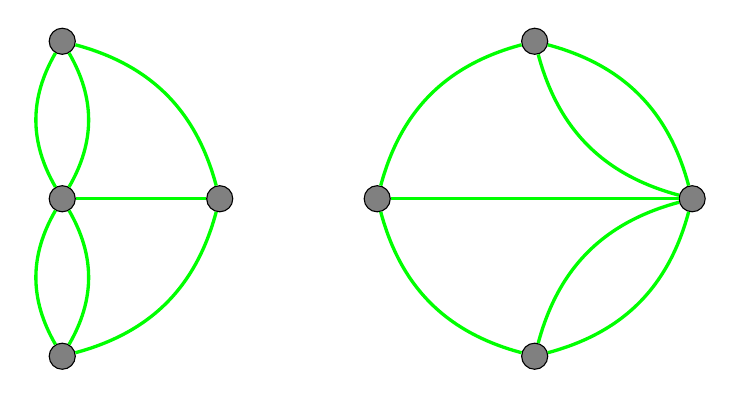
\begin{tikzpicture}
\node[shape=circle,draw=black,fill=gray](top) at (2,5) {};
\node[shape=circle,draw=black,fill=gray](midl) at (2,3) {};
\node[shape=circle,draw=black,fill=gray](midr) at (4,3) {};
\node[shape=circle,draw=black,fill=gray](bot) at (2,1) {};

\path[-] (top) edge[bend left,draw=green,very thick] (midl);
\path[-] (top) edge[bend right,draw=green,very thick] (midl);
\path[-] (midl) edge[bend left,draw=green,very thick] (bot);
\path[-] (midl) edge[bend right,draw=green,very thick] (bot);
\path[-] (midr) edge[bend right,draw=green,very thick] (top);
\path[-] (midr) edge[draw=green,very thick] (midl);
\path[-] (midr) edge[bend left,draw=green,very thick] (bot);

%

\node[shape=circle,draw=black,fill=gray](top2) at (8,5) {};
\node[shape=circle,draw=black,fill=gray](midr2) at (6,3) {};
\node[shape=circle,draw=black,fill=gray](midl2) at (10,3) {};
\node[shape=circle,draw=black,fill=gray](bot2) at (8,1) {};

\path[-] (top2) edge[bend left,draw=green,very thick] (midl2);
\path[-] (top2) edge[bend right,draw=green,very thick] (midl2);
\path[-] (midl2) edge[bend left,draw=green,very thick] (bot2);
\path[-] (midl2) edge[bend right,draw=green,very thick] (bot2);
\path[-] (midr2) edge[bend left,draw=green,very thick] (top2);
\path[-] (midr2) edge[draw=green,very thick] (midl2);
\path[-] (midr2) edge[bend right,draw=green,very thick] (bot2);
	\end{tikzpicture}
	\caption{Two graphified versions of The Seven Bridges of K\"onigsberg. The left graph is roughly a direct translation of the actual landmasses. The right graph is the same graph with the vertices moved around (take the middle-left vertex in the first graph, move it out to the left, then rotate the resulting graph 180 degrees)} \label{seven-bridges-graph}
\end{figure}

The beautiful thing about graphs is that we can move the vertices around in space, and so long as the edges remain connected to their respective vertices, without changing the fundamental structure of the graph!

Graphs are applicable in numerous fields, including
\begin{itemize}
	\item Network (computer, water, electric) flow
	\item Facebook friendships
	\item Google Maps path-finding
	\item E-commerce similarity predictions
	\item Neural networks
	\item \dots
\end{itemize}

\section{Key Terms}

\begin{defn}[Graph\index{Graph}]
	A set of abstract points, called vertices \(V\), and connections between those points, called edges \(E\). We denote a graph as \(G = \{V, E\}\) or \(G = (V, E)\). The order that you list \(V\) and \(E\) does not matter, however typically \(V\) is listed before \(E\)
\end{defn}

\begin{defn}[Vertex]

\end{defn}

\begin{defn}[Edge]
	Directed vs Un-directed
\end{defn}

\begin{defn}[Di-graph]
	A graph where each edge is directed.
\end{defn}

\begin{defn}[Cycle]
	A thing. Only defined for directed edges
\end{defn}

\begin{defn}[DAG]
	A Directed Acyclic Graph -- a di-graph with no cycles
\end{defn}

\section{Graph Representations}

There exist multiple ways to represent a graph. Each way has benefits and drawbacks. Typically algorithmic analysis involving graphs uses the representation that provides the best run-time.

\begin{defn}[Adjacency Matrix\index{Graph!Adjacency Matrix}]
	An \(m \times m\) (square) symmetric matrix \(M\) of 0s and 1s. Each row/column represents a node, and the position \(i,j\) in \(M\) represents the connection. For an edge 
\end{defn}

\section{Problems}

\section{Summary}

\section{Practice}

\end{document}
